% GNUPLOT: LaTeX picture with Postscript
\documentclass[20pt, border=0pt]{standalone}

\usepackage{graphicx}
\usepackage{xltxtra, xgreek}
\usepackage{alphabeta,csquotes}
\setmainfont{NewComputerModern10}
\fontsize{20}{12}\selectfont
\begin{document}


\begingroup
  \makeatletter
  \providecommand\color[2][]{%
    \GenericError{(gnuplot) \space\space\space\@spaces}{%
      Package color not loaded in conjunction with
      terminal option `colourtext'%
    }{See the gnuplot documentation for explanation.%
    }{Either use 'blacktext' in gnuplot or load the package
      color.sty in LaTeX.}%
    \renewcommand\color[2][]{}%
  }%
  \providecommand\includegraphics[2][]{%
    \GenericError{(gnuplot) \space\space\space\@spaces}{%
      Package graphicx or graphics not loaded%
    }{See the gnuplot documentation for explanation.%
    }{The gnuplot epslatex terminal needs graphicx.sty or graphics.sty.}%
    \renewcommand\includegraphics[2][]{}%
  }%
  \providecommand\rotatebox[2]{#2}%
  \@ifundefined{ifGPcolor}{%
    \newif\ifGPcolor
    \GPcolorfalse
  }{}%
  \@ifundefined{ifGPblacktext}{%
    \newif\ifGPblacktext
    \GPblacktexttrue
  }{}%
  % define a \g@addto@macro without @ in the name:
  \let\gplgaddtomacro\g@addto@macro
  % define empty templates for all commands taking text:
  \gdef\gplbacktext{}%
  \gdef\gplfronttext{}%
  \makeatother
  \ifGPblacktext
    % no textcolor at all
    \def\colorrgb#1{}%
    \def\colorgray#1{}%
  \else
    % gray or color?
    \ifGPcolor
      \def\colorrgb#1{\color[rgb]{#1}}%
      \def\colorgray#1{\color[gray]{#1}}%
      \expandafter\def\csname LTw\endcsname{\color{white}}%
      \expandafter\def\csname LTb\endcsname{\color{black}}%
      \expandafter\def\csname LTa\endcsname{\color{black}}%
      \expandafter\def\csname LT0\endcsname{\color[rgb]{1,0,0}}%
      \expandafter\def\csname LT1\endcsname{\color[rgb]{0,1,0}}%
      \expandafter\def\csname LT2\endcsname{\color[rgb]{0,0,1}}%
      \expandafter\def\csname LT3\endcsname{\color[rgb]{1,0,1}}%
      \expandafter\def\csname LT4\endcsname{\color[rgb]{0,1,1}}%
      \expandafter\def\csname LT5\endcsname{\color[rgb]{1,1,0}}%
      \expandafter\def\csname LT6\endcsname{\color[rgb]{0,0,0}}%
      \expandafter\def\csname LT7\endcsname{\color[rgb]{1,0.3,0}}%
      \expandafter\def\csname LT8\endcsname{\color[rgb]{0.5,0.5,0.5}}%
    \else
      % gray
      \def\colorrgb#1{\color{black}}%
      \def\colorgray#1{\color[gray]{#1}}%
      \expandafter\def\csname LTw\endcsname{\color{white}}%
      \expandafter\def\csname LTb\endcsname{\color{black}}%
      \expandafter\def\csname LTa\endcsname{\color{black}}%
      \expandafter\def\csname LT0\endcsname{\color{black}}%
      \expandafter\def\csname LT1\endcsname{\color{black}}%
      \expandafter\def\csname LT2\endcsname{\color{black}}%
      \expandafter\def\csname LT3\endcsname{\color{black}}%
      \expandafter\def\csname LT4\endcsname{\color{black}}%
      \expandafter\def\csname LT5\endcsname{\color{black}}%
      \expandafter\def\csname LT6\endcsname{\color{black}}%
      \expandafter\def\csname LT7\endcsname{\color{black}}%
      \expandafter\def\csname LT8\endcsname{\color{black}}%
    \fi
  \fi
    \setlength{\unitlength}{0.0500bp}%
    \ifx\gptboxheight\undefined%
      \newlength{\gptboxheight}%
      \newlength{\gptboxwidth}%
      \newsavebox{\gptboxtext}%
    \fi%
    \setlength{\fboxrule}{0.5pt}%
    \setlength{\fboxsep}{1pt}%
\begin{picture}(9070.00,9070.00)%
    \gplgaddtomacro\gplbacktext{%
      \csname LTb\endcsname%%
      \put(1460,1532){\makebox(0,0)[r]{\strut{}-1.0 $\pi \alpha$ }}%
      \put(1460,3043){\makebox(0,0)[r]{\strut{}-0.5 $\pi \alpha$ }}%
      \put(1460,4555){\makebox(0,0)[r]{\strut{}0.0 $\pi \alpha$ }}%
      \put(1460,6066){\makebox(0,0)[r]{\strut{}0.5 $\pi \alpha$ }}%
      \put(1460,7577){\makebox(0,0)[r]{\strut{}1.0 $\pi \alpha$ }}%
      \put(1580,1332){\makebox(0,0){\strut{}-1.0 $\pi \alpha$ }}%
      \put(3091,1332){\makebox(0,0){\strut{}-0.5 $\pi \alpha$ }}%
      \put(4602,1332){\makebox(0,0){\strut{}0.0 $\pi \alpha$ }}%
      \put(6113,1332){\makebox(0,0){\strut{}0.5 $\pi \alpha$ }}%
      \put(7624,1332){\makebox(0,0){\strut{}1.0 $\pi \alpha$ }}%
    }%
    \gplgaddtomacro\gplfronttext{%
      \csname LTb\endcsname%%
      \put(190,4554){\rotatebox{-270}{\makebox(0,0){\strut{}Y}}}%
      \put(4602,1032){\makebox(0,0){\strut{}X}}%
      \put(4602,7977){\makebox(0,0){\strut{}\Large Τιμή ροικής συνάρτησης και διανύσματα ταχυτήτων πεδίου}}%
      \csname LTb\endcsname%%
      \put(8197,1532){\makebox(0,0)[l]{\strut{}-1.0}}%
      \put(8197,2136){\makebox(0,0)[l]{\strut{}-0.8}}%
      \put(8197,2741){\makebox(0,0)[l]{\strut{}-0.6}}%
      \put(8197,3345){\makebox(0,0)[l]{\strut{}-0.4}}%
      \put(8197,3950){\makebox(0,0)[l]{\strut{}-0.2}}%
      \put(8197,4554){\makebox(0,0)[l]{\strut{}0.0}}%
      \put(8197,5159){\makebox(0,0)[l]{\strut{}0.2}}%
      \put(8197,5763){\makebox(0,0)[l]{\strut{}0.4}}%
      \put(8197,6368){\makebox(0,0)[l]{\strut{}0.6}}%
      \put(8197,6972){\makebox(0,0)[l]{\strut{}0.8}}%
      \put(8197,7577){\makebox(0,0)[l]{\strut{}1.0}}%
      \put(8857,4154){\rotatebox{-270}{\makebox(0,0){\strut{} \Large Τιμή ροϊκής συνάρτησης  \Large $\frac{\psi}{U_0 \alpha}$}}}%
    }%
    \gplbacktext
    \put(0,0){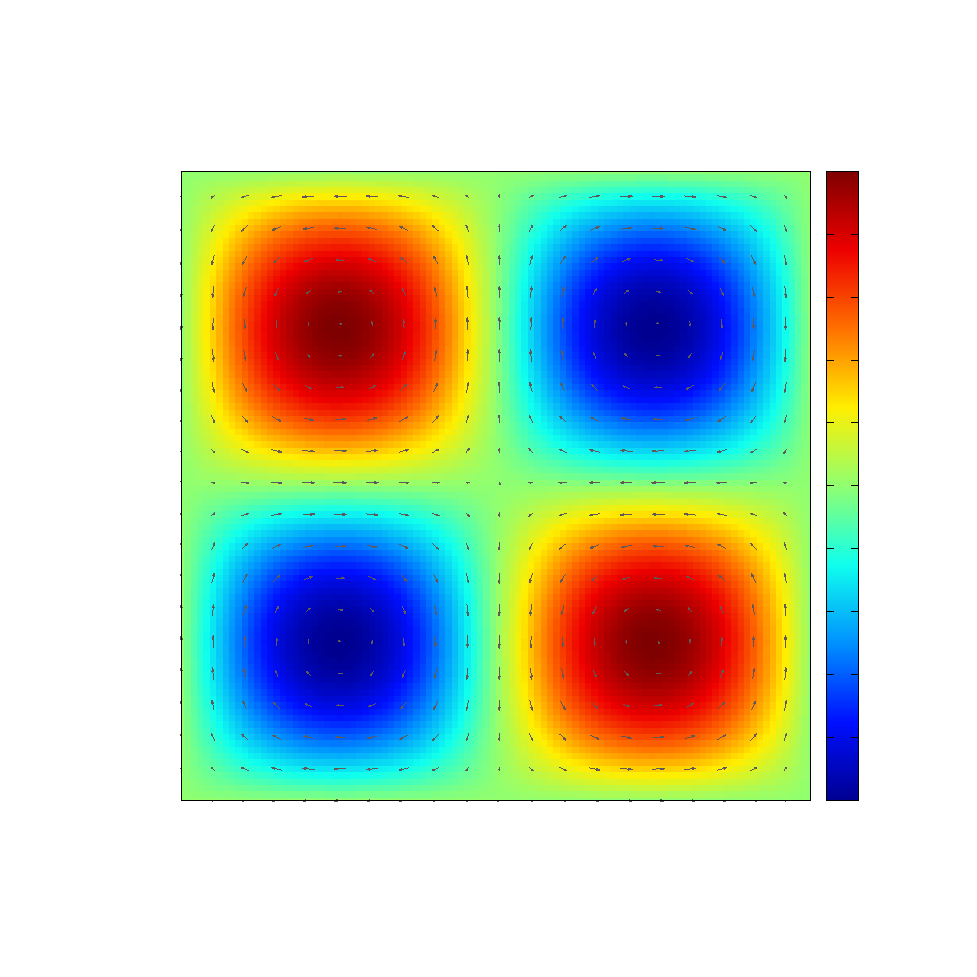
\includegraphics{roiki}}%
    \gplfronttext
  \end{picture}%
\endgroup
  
\end{document}